\documentclass{article}
\usepackage{apacite}
\usepackage{blindtext}
\usepackage{amsmath}
\usepackage{amssymb}
\usepackage{amsmath}
\usepackage[utf8]{inputenc}
\usepackage{bbm}
\usepackage[margin=1in]{geometry} % set margins
\usepackage{subcaption} % allows for subfigures
\usepackage{graphicx} % allow inclusion of figures/photos/pdfs
\usepackage{setspace} % allows changes between 
% \doublespacing \singlespacing \onehalfspacing
\onehalfspacing
\graphicspath{{./figure/}}
\usepackage[justification=centering]{caption}
\usepackage{cancel}
\usepackage{mathrsfs}

\usepackage{Sweave}
\begin{document}
\Sconcordance{concordance:Dilgin_MPSA.tex:Dilgin_MPSA.Rnw:%
1 19 1 1 0 133 1 1 11 31 1}

	\title{Where to Spend the Money? A Survey Experiment on Electoral Institutions and Party Expenditure at the District Level}
	\author{Tolgahan Dilgin}
	\date{03/28/2018}
	\maketitle
	
\begin{abstract}
This paper is part of dissertation research that examines the impact of electoral institutions on how political parties choose to engage in vote buying practices at the district level. Regardless of electoral rules, parties tend to concentrate their vote buying spending in the most competitive districts as opposed to party strongholds in order to maximize their electoral gains. This research argues that Proportional Representation (PR) systems enable political parties distribute their vote buying activities more evenly between party strongholds and competitive districts in comparison to Single Member District (SMD) systems. In the face of difficulty in testing this theory empirically, the paper takes advantage of the unique political structure of Mexico, which uses both SMD and PR systems in its elections. The survey experiment with Mexican students -who are exposed to both of the systems- seems to provide evidence consistent with paper's main theoretical claim.
\end{abstract}

\section{Introduction}
The consequences of electoral systems have been a widely debated topic in political science for several decades. The argument that Proportional 
Representation performs better on several aspects of democratic life goes back to John Stuart Mill's Considerations on  Representative Government \cite{mill1861considerations}. Likewise, the study of why several European countries shifted from Single Member District (SMD) system to Proportional Representation in Europe goes as early as 1930s \cite{braunias1932parlamentarische} and has been revisited recently frequently by scholars from 1970s onward \cite{rokkan_citizens_1970, boix_setting_1999, cusack_economic_2007}. Ever since, the scholarly work has made important advances on our knowledge on how electoral institutions may have come into being, and how they may help us explain certain political phenomena.\\
\iffalse
I made a reference to mill from Becher article.It says Chapter 7. Double-make sure that this is the case. I ordered the book online.
\fi
\\
Perhaps, our most widely accepted piece of knowledge is that the choice of electoral systems brings certain trade-offs such as the one between accountability and representation \cite{diamond1999developing,carey_electoral_2011,persson_economic_2003,britain1998report}.In countries with Proportional Representation systems, each district in a country elects multiple representatives which allows different political opinions to be heard both at the local and national assemblies. The advantage of this system is that it gives a voice to minority opinions without allowing them to be crushed by the choices of majorities at the district or national levels. The downside is that when voters are not happy with how things are at their district, it is hard for them to pinpoint \textit{the} responsible person, as all representatives will be pointing each other. \\
\\
Scholars argue that there are several other trade-offs in the electoral choices countries make between these two systems. For instance, majoritarian systems are argued to bring strong and effective governments, whereas proportional systems are likely to bring coalition governments from smaller parties that may or may not work in harmony \cite{norris1997choosing}. There is also the trade-off between inclusiveness and fairness to minor parties vs. vertical accountability and accessibility of a system\cite{norris1997choosing, diamond1999developing}. One could easily argue that proportional systems harbor a greater number of parties representing ethno-religious minorities, whereas majoritarian systems would offer clearer picture of accountability in the vertical structure of a government and accessability to one single representative at each district \cite{norris1997choosing, diamond1999developing}. \\
\\
Another dimension of possible trade-offs is pertinent to the responsiveness of policy makers. Smaller swings in the vote may bring greater changes in the total seat share in a majoritarian system due to the disproportionality of this system that generally favor the winner. That is, if there is a 2-3 percent vote change at the national level, this may bring majority of seats to the the opposition, thereby a change in the government. For that reason, the incumbent government has greater incentive to be responsive to the change in the public opinion and policy demands \cite{norris1997choosing}. On the other hand, the districts may have a different dynamic due to the winner-takes-all attribute of majoritarian systems. For instance, if a representative comes from party stronghold district, lagging responsiveness would be less punishable, as there is a strong ideological leaning toward incumbent's party and the opposition is inherently unpopular regardless of their policy offerings. One could argue that PR creates more responsive candidates at the district level, as voters will have more choices amongst the candidates.\\
\\
This study will examine the possibility of a different trade-off at the district level by raising the question of how electoral rules may influence the way in which parties spend their resources. Particularly, this paper focuses on the trade-off between choosing one electoral rule versus another in terms of prevalence of campaign spending (that may include campaign ads and vote buying) at the district level.\\
\\
This brings an important question: which kind of electoral rules make some districts targeted by the foul practices that diminish the democratic accountability. As Stokes (2005) famously put forward, it is perverse accountability for political parties to monitor and retaliate on the behavior of voters for not voting for them, as different forms of vote buying and clientelism aim to achieve \cite{stokes_perverse_2005}. If there is any way for political scientists to make connections between electoral rules and how political parties will spend their resources on activities such as campaign ads and vote buying, that would enhance our understanding about not only how democratic institutions should (and should not) work in a society, but also what kinds of trade-offs we face when making choices between electoral institutions in new democracies.\\
\\
With these considerations in mind, the paper investigates the interplay between electoral institutions and campaign spending by raising the following question: How do electoral rules affect the way political parties engage in vote buying in certain districts versus others under different electoral systems? I argue that winner-takes-all structure of SMD systems cause parties to focus more on the competitive districts that they would otherwise (i.e. under PR systems) do, given the high stakes of losing. Similarly, in non-competitive districts, parties do not need to invest much in their constituency regardless of whether they are either winning or losing. Conversely, PR systems allow losers to gain seats and there is always a seat to compete for the losing party even in its competitor's stronghold district.\\
\\
A challenge in empirically testing this theory comes from the fact that this comparison involves a difficult to identify counterfactual. The ideal comparison would have been to analyze the distribution of party expenditure across districts under one system first, and then go back in time, change the electoral system, and observe how differently parties would make their expenditure decisions in the same country. Unfortunately, real world data almost never allows this type of 'perfect' comparison, and thus researchers end up comparing different countries under different electoral systems. \\
\\
This study, however, aims to overcome this comparability issue without falling into the trap of comparing different countries' data. With that in mind, it makes use of an original survey experiment, where half of the respondents are given the PR treatment, whereas the other are given the SMD treatment. These surveys were conducted in Mexico and the US. \\
\\
The reason for conducting the survey in Mexico is because this country uses both the PR and SMD systems in its legislative elections. The mixed nature of the electoral system creates an environment where voters are exposed to both systems, and therefore would be responsive to both PR and SMD treatments in a survey experiment. Arguably, student in the US (Argentina), which uses SMD (PR) system only in its legislative elections, would not be responsive to the PR (SMD) treatment if the survey was conducted in the US (Argentina). In order to minimize this disadvantage in the US data, the paper took measures such as filtering out the students who were not knowledgeable on the difference between the two electoral institutions. These measure will be discussed more in detail in the coming sections.

\section{Theoretical Considerations}
This paper argues that political parties tend to spread their vote buying expenditure across districts more equally under Proportional Representation (PR) systems\footnote{Under Proportional Representation systems, each district has multiple seats that are distributed between parties in proportion to their vote share at that district.} in comparison to Single Member District (SMD) systems.\footnote{Under Single Member District systems, each district has only one seat that goes to the political party or candidate who has won either majority (more than half of the total vote) or plurality (the greatest vote share.) Depending on the electoral formula, there may be cases where there are multiple contenders vying under a majoritarian system, where no single candidate receives the majority (but plurality) of vote. In these cases, elections go to a second round where only the first two candidates compete.} The main mechanism behind this claim comes from the fact that districts in an SMD system elect only one winner, which makes the stakes of winning and losing very high for all contenders. SMD systems often determine the winners by either plurality or majority rule, and this means that a candidate with either majority (50\% + 1 vote) or plurality (the greatest share of votes amongst multiple competitors) will end up getting 100\% of representation of that district (i.e. they will win the sole representative of the entire district.) This means that strong parties will almost certainly win the electoral competition in that district. On the flip side of the coin, SMD systems also bring tremendous difficulty for the weaker parties who are trying to penetrate districts where their rival has a strong support base. As SMD systems bring high entry costs for the underdog parties in winning parties’ strongholds, this creates little to no incentive for non-winning parties to engage in activities such as campaign ads or vote buying in the stronghold of their competitors. That is, competitive districts receive more party expenditure (than they would have under PR), whereas strongholds do not under SMD systems (although they do under PR systems.)\\ 
\\
On the other hand, PR systems do not offer such a clear-cut picture. When there are multiple seats in a district where seats are distributed relatively in proportion to each party’s vote share, even if party A has a strong support, party B may still have an incentive to compete in that district in the hope that it would at least win 1 or 2 of those multiple seats. This creates a tendency in PR systems for parties to invest their resources in other parties' strongholds so that they can achieve small portions of representation in these districts. This tendency opens a door for weaker parties to penetrate the strongholds of their rivals. In the face of lower entry costs for the underdog parties, the strong parties in that district would also tend to spend more money for their supporters under PR systems than they would have under SMD systems.\\
\\
This would mean that there would be greater variance in SMD systems in terms of how much of their limited resources parties choose to spend on activities such as campaign ads and vote buying. In districts where there is a strong support for any party, both the winning party and its rival would have fewer incentives to invest their resources in that particular district. In districts where there is more uncertainty about the possible winner, parties may channel their resources due to the winners-take-all nature of single member districts. In line with this logic, the entry to the rival parties' basis of support would be easier in districts under a PR system, and there would be a more heterogeneous distribution of vote buying behavior. With this mechanism in mind, I propose to test the following proposition:\\
\\
\textit{\underline{Proposition 1:} Campaign spending will be more equally distributed across districts under PR systems than they are under SMD systems. (Countries with SMD systems will have greater variance in their campaign spending across districts in comparison to countries with PR systems.)}\\
\\
The following typology may be useful in visualizing the main argument and what I mean by parties' involvement in strategizing their campaign spending.
\begin{center}
	\begin{tabular}{ |c|c|c| } 
		\hline
		 & Competitive & Stronghold \\ 
		\hline
		SMD & a & d \\ 
		\hline
		PR & b & c \\ 
		\hline
	\end{tabular}
\end{center}\\
\\
In line with Proposition 1, the paper's theory can be summarized as $a>b>c>d$. This concise theory lends itself to a number of hypotheses. First, I argue that competitive districts tend to receive more vote buying (denoted by $a>d$ and $b>c$), which is a claim that is largely backed by our conventional wisdom in comparative politics. The novel argumentation in the theory comes from the part that focuses on differences that occur in the level of vote buying \textit{across different electoral systems} ($a>b$ and $c>d$). In sum, I argue that electoral systems have an impact on how campaign spending is organized at the district levels. The argument is that political parties ``strategize'' their vote buying efforts at the district level more under Single Member Districts than they do in Proportional Representation. 

\section{Background and Literature Review}
The research on the interplay between electoral institutions and vote buying has been limited to a number of qualitative studies that focus on clientelism in country case studies. In one such study, Kristinsson (2001) states that electoral systems change in Iceland caused a decline in the practice of clientelism. When Iceland introduced proportional representation in 1959, this brought a more equal weight across the districts in terms of their seats-votes ratios. This was mainly due to the fact that this increased the weight of districts in which people were least favorable against existing clientelism. For instance, 46 percent of the constituency in Reykjavik (the capital of Iceland) had stated in an opinion poll that they were against clientelism as opposed to the 31 percent in the provincial constituencies. Therefore, the increased weight of Reykjavik districts in determining the distribution of legislative seats meant that electoral system change responded more to the public opinion against clientelism (Kristinsson, 2001). Kristinsson states that the new electoral system in Iceland also lowered the electoral threshold, which meant that a greater number of parties were able to receive legislative seats after the elections. Kristinsson states that almost all of these new parties in the system made ``ethics in government'' an issue in their campaigning, which increased the risk for political parties to engage in clientelism when the general opinion was turning very much against its practice \cite{kristinsson2001clientelism}.\\
\\
In another study with similar approach, M\"uller makes case study comparisons of possible influences of electoral rules in different countries. After discussing a number of theories that may be explaining the interaction between electoral settings and clientelism, he concludes that the influence of electoral institutions should not be overestimated (M\"uller, 2007).\\
\\
According to Scheiner, there were two mechanisms that made the Japanese electoral rules more conducive to clientelistic practices. First one was the system of Single Non-Transferable Vote in Multi-Member Districts (SNTV/MMD). This is a system where the total cast for one particular candidate cannot be transferred to another candidate within the same party, even when these two candidates compete in the same electoral district. Scheiner argues that this created an environment for candidates to invest more in clientelism in order to attract more votes for themselves (Scheiner 2007; see also Carey and Shugart 1995). That is, SNTV/MMD creates intra-party competition between candidates even under the same party. This, he argues, makes ``clientelistic distribution of goods a logical strategy'' (Scheiner 2007). Accordingly, candidates have to differentiate themselves from one another by channeling government money or resources to voters and interest groups\footnote{More precisely, he claims that ``the evidence suggests that Liberal Democratic Party (LDP) same-district incumbents differentiated themselves from one another by providing particularistic government resources to different organized interests (McCubbins and Rosenbluth 1995) or geographical regions (Tatebayashi and McKean 2002).'' (Scheiner 2007).}.\\
\\
This paper will follow a different empirical approach from the previous authors. Instead of a qualitative country-case study, I will analyze empirical data collected from political science students who are also at the voting age in Mexico- a country that uses both of the electoral systems in its legislative elections. This way, I will have higher chances that the treatments I give to the respondents (PR rules versus SMD rules) will be effective, as they will be exposed to these rules both through their formal training at their university and their exposure to Mexican political institutions as voting age citizens that has just experienced a major legislative elections and a government change in the previous months to my visit to Mexico in summer 2018\footnote{I thank my funding institution Center for Latin American and Caribbean Studies (CLACS) at the University of Illinois for their generous support to this project.}. In addition, I will combine this dataset with the political science students at University of Illinois\footnote{Since the US uses SMD system, I will follow a different strategy with the US sample in terms of filtering out respondents with effective treatments}. 
\section{Research Design}
This paper will use two survey experiments that were conducted in September 2018 in Mexico and December 2018 in the US. The reason for the use of survey experiments come from the fact that many of my concepts in the theory section are interconnected with one another. To be more specific, electoral institutions have an impact on the size and number of districts in a country. SMD systems tend to consist of a larger number of smaller districts, whereas PR systems have a smaller number of districts that are greater in size. Another relationship that is hard to disentangle is the electoral systems' influence on the size and number of political parties. SMD systems are more likely to induce two big parties at the national level, whereas PR systems will be more likely to accommodate a higher number of political parties (Duverger, 1954).\\
\\
In my research design, however, these were not major concerns, as I was able to limit the number of political parties to two, and kept both the district number and size equal in both systems. By isolating certain parts of electoral systems, survey experiments enabled me to make the right comparison between size of expenditure across equally sized districts where an equal number of parties are competing, hence, enabled me to tease out the impact of electoral institutions on the expenditure. In sum, with the ability to manipulate the number of parties and districts along with size of districts in the system, a survey experiment proved to be an appropriate method due to its controlled environment making a comparison between districts possible.

\subsection{Survey Experiment with University Students in Mexico and United States}
In the survey experiment with political science students both in Mexico and the United States (US), I asked respondents to form electoral strategies before elections in the scenario that they were working as a consultant for a political party. The main advantage of having this experiment in Mexico was that this is a distinctive country in the Latin American region that uses both SMD and PR systems at its legislative elections. Thus, respondents are exposed to the workings of both systems, whereas arguably a concern in the American sample would be that PR treatment will not be effective as students are only exposed to SMD system.  For that reason, I took extra measures with the US sample.\\
\\
As the electoral system in the US is SMD, American respondents are highly likely not to know how PR systems work in legislative elections of other countries. Similarly, political science students at UIUC may exclusively focus on American politics, and may not have training on how the PR systems work around the world. Due to this lack of exposure, I decided to screen out the students who did not know the difference between SMD and PR through a political knowledge question in our background survey. I also asked students to identify their treatment after the survey\footnote{Electoral rules in this game ... [Complete](Option A: gave the sole seat in a district to the party that received more than 50 \% of the vote Option B: gave the seats in a district to parties in proportion to their vote share Option C: I don't know/I'm not sure)}. If the students were not able to answer this question correctly, I took them out of my sample.\footnote{This was not possible in the print surveys with Mexican students, where students would have the option to go back to the previous page and check the treatment. The survey in the US was online, so students did not have an option to go back to check the treatment. }\\
\\
In the survey, I asked the respondents to imagine that they are a political consultant for a political party in the imaginary country of Hawaisteros. I stated that they have been hired to help the party win the elections. I stated that there are 9 districts in Hawaisteros: 3 are their party's strongholds, 3 are competitive districts, and last 3 are rival party's stronghold. I assigned each respondent 100,000 Lingots (the local currency of Hawaisteros) and asked them to distribute this amount across the 9 districts in a way that they think would maximize their chance to win this political game\footnote{See Appendix for the full text of the treatment, and the question measuring the effect of the treatments}.\\
\\
\subsection{Research Findings}
This section will discuss the empirical findings from the survey experiment I conducted in the US and Mexico in light of my theoretical expectations. Proposition 1 had argued that the relationship between these four types of districts should be $a>b>c>d$. As discussed previously, this means that competitive districts tend to receive more vote buying than non-competitive or stronghold districts ($a>d$ and $b>c$). The proposition also puts forward a second set of hypotheses that the gap between districts will be higher under SMD than they are under PR systems ($a>b$ and $c>d$). The following boxplot data that includes all the respondents pooled together helps see the preliminary results  support the theory.\\
\\
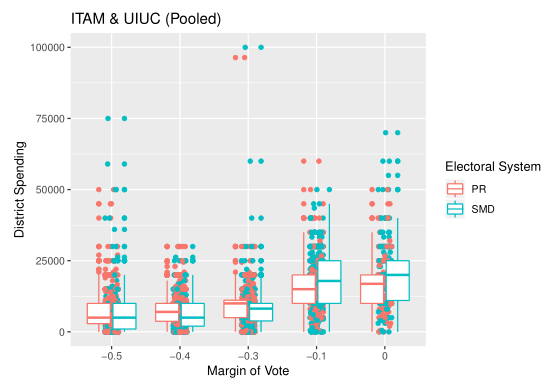
\includegraphics[width=120mm]{Boxplot_Pooled}
\\
In the graph, the horizontal axis indicates the level of competition measured by the margin of vote that was given to the respondents. When forming this variable, I took the absolute values of the vote difference in percentages between the winning and losing parties, and multiplied this by $-1$ so that the more competitive districts will be on the right-hand side. In party strongholds we see that PR averages are either equal or more than the SMD averages, whereas in competitive districts we see that majoritarian districts tend to receive more campaign spending that PR in line with the theory.\\
\\
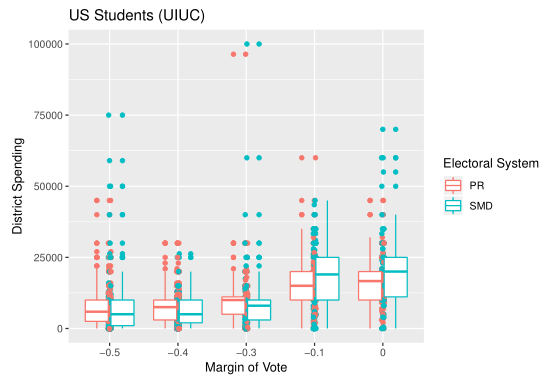
\includegraphics[width=90mm]{Boxplot_UIUC}
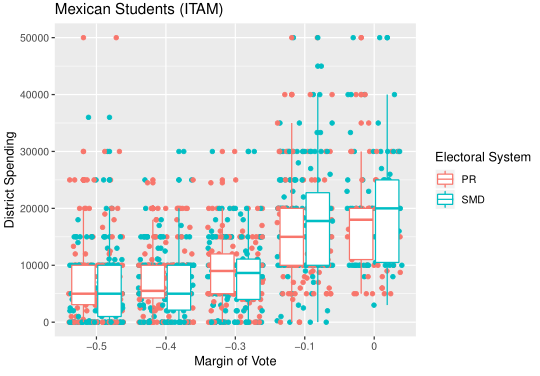
\includegraphics[width=90mm]{Boxplot_ITAM}\\
When we look at the individual samples, they are largely simmilar. In competitive districts SMDs tend to get more spending, whereas they do receive less or equal spending in strongholds. The only difference from the pooled data is that the equality in districts with 50\% margin disappears in the UIUC data in favor of the theory. Upon the visual inspection of descriptive statistics, we may also look whether these seeming differences between means are statistically meaningful. \\
\\
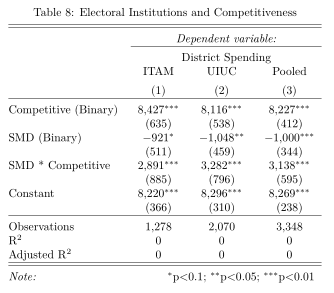
\includegraphics[width=90mm]{Regressions_All}\\
\\
In order to test the hypothesis, I conducted a simple regression model\footnote{Ordinary Least Squares (OLS) with robust standard errors} from the data combined the students from University of Illinois in the US, and Instituto Tecnol\'{o}gico Aut\'{o}nomo de M\'{e}xico (ITAM) in Mexico. This means calculation of predicted values would be as follows:\\
\begin{center}
	\begin{tabular}{ |c|c|c| } 
		\hline
		 & Competitive & Stronghold \\ 
		\hline
		SMD & 18,634 & 7,269 \\ 
		\hline
		PR & 16,496 & 8,269 \\ 
		\hline
	\end{tabular}
\end{center}\\
\\

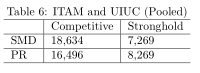
\includegraphics[width=70mm]{Coefficients_Pooled}\\
\\
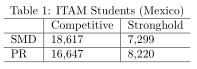
\includegraphics[width=70mm]{Coefficients_ITAM}\\

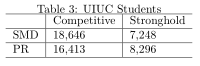
\includegraphics[width=70mm]{Coefficients_UIUC}\\
\\
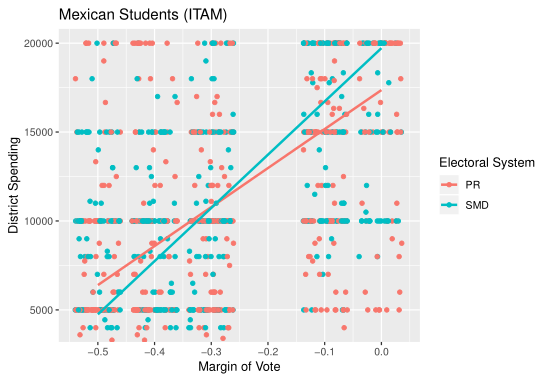
\includegraphics[width=120mm]{Interactive_ITAM}\\
\\
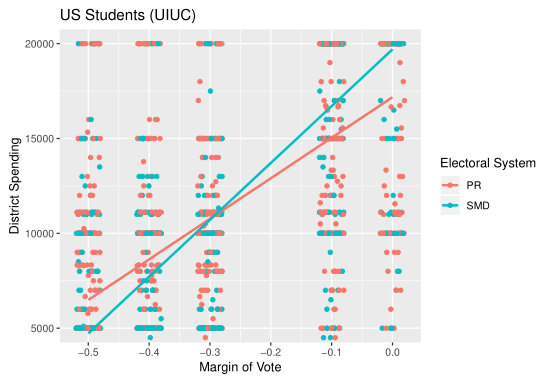
\includegraphics[width=120mm]{Interactive_UIUC}\\

\iffalse
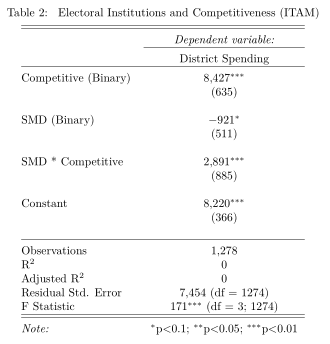
\includegraphics[width=90mm]{Regressions_ITAM}\\
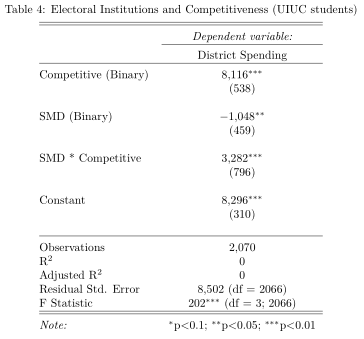
\includegraphics[width=90mm]{Regressions_UIUC}\\
\fi


\\





\bibliographystyle{apacite}
\bibliography{MPSA_References}

\section{Appendix} 
The following visual shows a randomly selected nine respondents' responses to the question, where the horizontal axis shows the vote margin as a competitiveness measure and vertical axis is the spending in that district:\\
\\
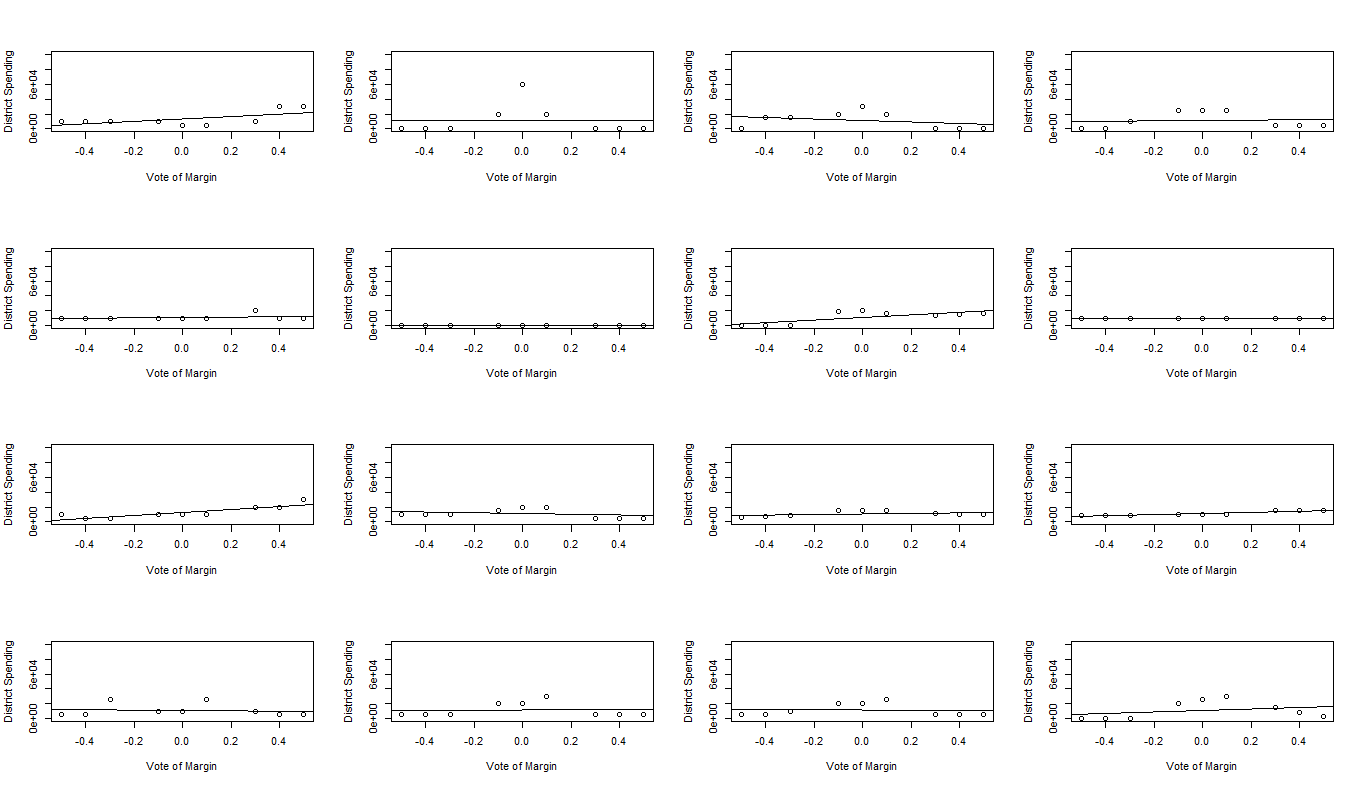
\includegraphics[width=180mm]{Respondents_1}
\\

\iffalse the trade-off
Matt's PS 345 slide. 
Electoral System Design: Four Normative Trade-offs (Diamond 1999)
-Efficiency/Governability vs. Representativeness
-Representativeness/Inclusiveness vs. Vertical Accountability/Accessibility 
-Party Coherence vs. Voter Choice
- Simplicity/Ballot Accessibility vs. Appropriateness of System to Country

--
Actual, Diamond 1999- Developing Democracy: Toward Consolidation p.100
"Four normative trade-offs become salient in designing (or reforming) electoral systems for contemporary democracies"
Efficiency \&  vs. representativeness
"The more majoritarian the electoral system, the greater the distortion (disproportionality) between votes and seats, and the less representative the outcome (in giving parliamentary place voice to all interests and views.) However, the efficiency of democracy, "the ability of elections to serve as a means for voters to identify and choose among the competing government options available," is best served with a majoritarian electoral system, which can provide coherent governing alternatives known to the electorate in advance (ideally between two parties) and also a governing majority (footnote 94)."

Representativeness \& inclusiveness (PR) vs. direct vertical accountability \& accessibility (SMD system)

\fi


\end{document}
